%======================================================================
% 附录O：电推进：把等离子体当发动机（注明出处）
%======================================================================
% 章标题 \appchapter{附录O：...} 由主文件发出，本文件只提供正文。
% 设计约定：补"应用侧"的空白——第 3 章的 E×B 漂移、第 6 章的波与加热、第 11 章的鞘层在航天电推进里的合流。
% 版权约定：只借鉴经典教材与文献的物理结论、公式形式与题型，文字与数值由本书自拟并独立复算。
% 数值来源：tools/calc/appO_calc.py（本附录每一节的关键数字都能由它复现）。

第 3 章讲了 $\mathbf{E}\times\mathbf{B}$ 漂移，第 6 章讲了波与加热，第 11 章讲了鞘层与玻姆判据——这三块知识在航天领域有一个直接的去处：\textbf{电推进}（electric propulsion）。它的想法很朴素：与其用化学燃烧的热速度排气，不如\textbf{用电场把离子加速到几十千米每秒}。代价也同样朴素：同样的功率下，排气越快，推力越小。本附录把这条“把等离子体当发动机”的链条算一遍。

这一篇换到\textbf{应用侧}：不让等离子体待在容器里，而是让它喷出去产生推力：电推进、VASIMR 与磁喷嘴。想读书单、范例与自测题，翻配套手册 J、K、L；加热与运行极限在附录 M，边界与壁在附录 N。

\begin{tip}{单位与口径自查}{tip-appo-units}
若结果差一个量级，先查三种口径错位：
\begin{enumerate}[nosep,leftmargin=1.6em]
  \item 比冲 $I_{\mathrm{sp}}$ 的单位是“秒”（$I_{\mathrm{sp}}=v_{\mathrm{ex}}/g_0$）还是“$\mathrm{m/s}$”（那就是排气速度本身），两者差 $g_0=9.80665\ \mathrm{m/s^2}$；
  \item 推力是\textbf{束流推力} $T=I_b\sqrt{2m_iV_b/q}$ 还是含中性损失与羽流发散的\textbf{实测推力}（后者更小）；
  \item 功率是\textbf{束功率} $P_{\mathrm{jet}}=I_bV_b$ 还是\textbf{输入功率} $P_{\mathrm{in}}=P_{\mathrm{jet}}/\eta$（后者更大，$\eta$ 常只有 $0.5$--$0.7$）。
\end{enumerate}
另：公式里的时间单位一律写作 \texttt{yr}（年）与 \texttt{day}（天）；氙离子取 $m_{\mathrm{Xe}}=131.29\ \mathrm{u}=2.180\times10^{-25}\ \mathrm{kg}$。
\end{tip}


\section{为什么用电推进：比冲与火箭方程}

火箭能拿到多少速度增量，由齐奥尔科夫斯基公式给出：
\begin{equation}
\Delta v=v_{\mathrm{ex}}\ln\frac{m_0}{m_f},
\qquad
I_{\mathrm{sp}}\equiv\frac{v_{\mathrm{ex}}}{g_0},
\label{eq:app-o-rocket}
\end{equation}
其中 $v_{\mathrm{ex}}$ 是排气速度，$m_0/m_f$ 是初末质量比，$I_{\mathrm{sp}}$ 就是\textbf{比冲}——它把“排气多快”折算成一个以秒为单位的数。化学发动机的排气速度受化学键能限制，最高约 $4.5\ \mathrm{km/s}$（$I_{\mathrm{sp}}\approx450\ \mathrm{s}$）；而电推进先电离、再用电场加速，离子的动能 $\frac12m_iv^2=qV$ 只受电压限制，$1000\ \mathrm{V}$ 就能给出 $38\ \mathrm{km/s}$。

\begin{table}[htbp]
\centering
\small
\caption{同样的速度增量，比冲决定了要带多少推进剂（取 $\Delta v=10\ \mathrm{km/s}$）}
\label{tab:app-o-isp}
\begin{tabular}{@{}lrrrr@{}}
\toprule
发动机类别 & $I_{\mathrm{sp}}$（$\mathrm{s}$） & $v_{\mathrm{ex}}$（$\mathrm{km/s}$） & $m_0/m_f$ & 推进剂质量分数 \\
\midrule
化学（肼类/氢氧） & 450 & 4.41 & 9.64 & $89.6\%$ \\
霍尔推力器 & 1800 & 17.7 & 1.76 & $43.3\%$ \\
离子推力器（静电栅极） & 3000 & 29.4 & 1.40 & $28.8\%$ \\
磁等离子体（VASIMR 级） & 5000 & 49.0 & 1.23 & $18.4\%$ \\
\bottomrule
\end{tabular}
\end{table}

\textbf{一个具体例子。} $1000\ \mathrm{kg}$ 的卫星要拿到 $\Delta v=3\ \mathrm{km/s}$：用 $I_{\mathrm{sp}}=300\ \mathrm{s}$ 的化学发动机需要 $639\ \mathrm{kg}$ 推进剂（占起飞质量的 $64\%$）；换成 $I_{\mathrm{sp}}=3000\ \mathrm{s}$ 的电推进只需要 $97\ \mathrm{kg}$，省下的 $542\ \mathrm{kg}$ 可以换成载荷。

结论：\textbf{同样的 $\Delta v$，化学发动机要带走 $9.6$ 倍于自身的初始质量，而 $5000\ \mathrm{s}$ 的电推进只要 $1.23$ 倍}——这就是电推进存在的理由，也是它必须付出的代价：推力极小（下一节量化）。

{\footnotesize
\textbf{出处：}Sutton \& Biblarz《Rocket Propulsion Elements》（第 9 版）的火箭方程与比冲章节。
Jahn《Physics of Electric Propulsion》第 1 章的推进方式分类。
}


\section{推力与功率账：$40\ \mathrm{mN/kW}$ 的价目表}

推力来自动量流率，功率来自动能流率：
\begin{equation}
T=\dot m\,v_{\mathrm{ex}}=\dot m\,g_0I_{\mathrm{sp}},
\qquad
P_{\mathrm{jet}}=\frac12\dot m v_{\mathrm{ex}}^2=\frac12Tv_{\mathrm{ex}},
\qquad
\eta\equiv\frac{P_{\mathrm{jet}}}{P_{\mathrm{in}}}.
\label{eq:app-o-thrust}
\end{equation}
把 $v_{\mathrm{ex}}=g_0I_{\mathrm{sp}}$ 代入 $T/P_{\mathrm{in}}$，得到一个\textbf{与推力无关}的比值：
\begin{equation}
\frac{T}{P_{\mathrm{in}}}=\frac{2\eta}{g_0I_{\mathrm{sp}}}
\ \ \Longrightarrow\ \
I_{\mathrm{sp}}=3000\ \mathrm{s},\ \eta=0.6\ \text{时}\ \ \frac{T}{P_{\mathrm{in}}}=40.8\ \frac{\mathrm{mN}}{\mathrm{kW}}.
\label{eq:app-o-tpratio}
\end{equation}

\begin{table}[htbp]
\centering
\small
\caption{推力-功率账（$\dot m$ 为推进剂流量，$P_{\mathrm{in}}$ 为电源输入功率）。前两行取 $I_{\mathrm{sp}}=3000\ \mathrm{s}$、$\eta=0.6$，$T$ 分别为 $0.1\ \mathrm{N}$ 与 $10\ \mathrm{N}$；第三行是公开报道的 NSTAR 级指标（$I_{\mathrm{sp}}=3100\ \mathrm{s}$、$\eta=0.61$）}
\label{tab:app-o-tp}
\begin{tabular}{@{}lrrrrr@{}}
\toprule
工况 & $T$（$\mathrm{N}$） & $\dot m$（$\mathrm{mg/s}$） & $P_{\mathrm{jet}}$（$\mathrm{W}$） & $P_{\mathrm{in}}$（$\mathrm{W}$） & $T/P_{\mathrm{in}}$（$\mathrm{mN/kW}$） \\
\midrule
小推力 & 0.1 & 3.40 & 1471 & 2452 & 40.8 \\
大推力 & 10 & 339.9 & $1.47\times10^{5}$ & $2.45\times10^{5}$ & 40.8 \\
NSTAR 级 & 0.092 & 3.03 & 1398 & 2293 & 40.1 \\
\bottomrule
\end{tabular}
\end{table}

第三行是用公开报道的指标（约 $92\ \mathrm{mN}$、$2.3\ \mathrm{kW}$、$3100\ \mathrm{s}$、$61\%$）反算的，得到的 $P_{\mathrm{in}}=2293\ \mathrm{W}$ 与“$2.3\ \mathrm{kW}$”对得上，说明这套口径没有错位。要把 $10\ \mathrm{N}$ 的推力连续推一整年，需要
\begin{equation}
\dot m\times1\ \mathrm{yr}=3.40\times10^{-4}\times3.156\times10^{7}\approx1.07\times10^{4}\ \mathrm{kg}=10.7\ \mathrm{t/yr}.
\end{equation}
（注意这里用的是\textbf{日历秒}：推进剂的消耗按日历时间计；附录 N 里的“每年”指的是每年约 $10^{5}\ \mathrm{s}$ 的等离子体放电时间，两者口径不同，不能混用。）

结论：\textbf{推力与功率成正比（$40\ \mathrm{mN/kW}$）：想要 $1\ \mathrm{N}$ 就得准备 $24.5\ \mathrm{kW}$，想要 $100\ \mathrm{N}$ 需要 $2.45\ \mathrm{MW}$}——电推进因此只能做“长期小推力”，用时间换速度增量。

{\footnotesize
\textbf{出处：}Goebel \& Katz《Fundamentals of Electric Propulsion》的推力/功率/效率关系与推力器指标章节。
}


\begin{figure}[htbp]
\centering
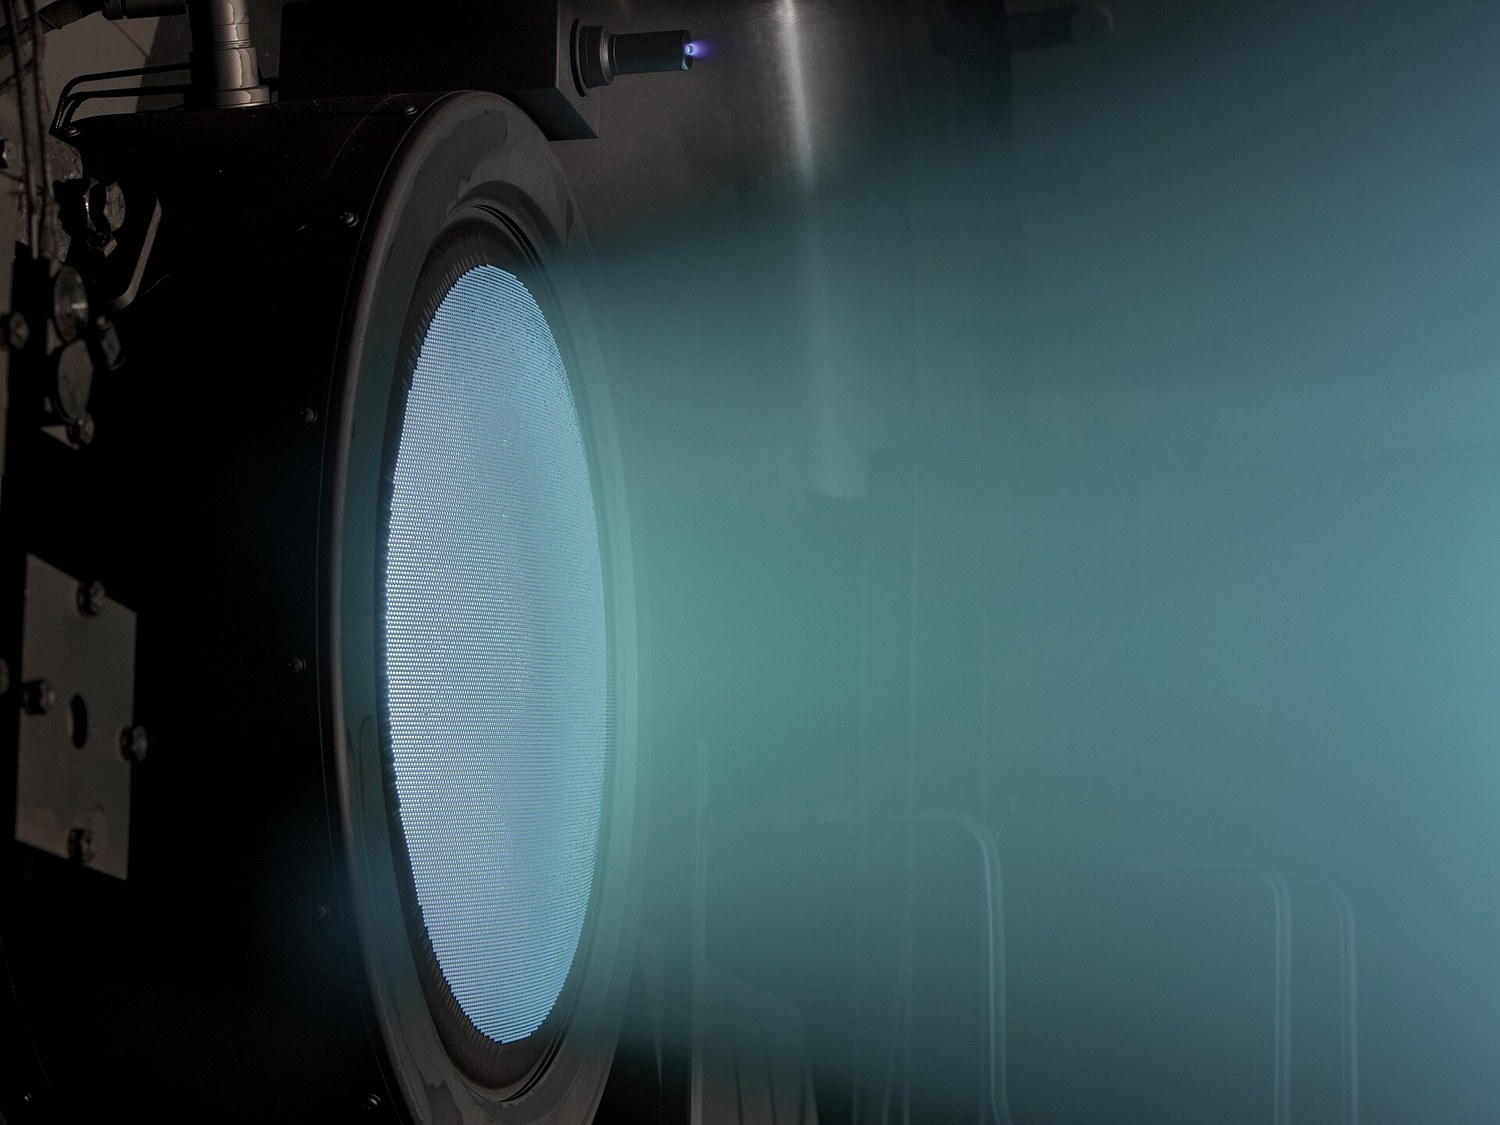
\includegraphics[width=0.72\textwidth]{../figures/o_ion_thruster.jpg}
\caption{NEXT 离子推力器：栅极把电压变成速度。静电加速的全部机构就是两层栅极：离子在几千伏的电位差里被加速，比冲因此可以做到化学火箭的十倍。}
\label{fig:photo-appo2}
\figsource{NASA，Public domain（Wikimedia Commons）}
\end{figure}

\section{静电加速：把电压变成速度}

单个离子的能量方程给出排气速度：
\begin{equation}
\frac12m_iv^2=qV
\qquad\Longrightarrow\qquad
v=\sqrt{\frac{2qV}{m_i}} .
\label{eq:app-o-vbeam}
\end{equation}
若束流为 $I_b$，则质量流率 $\dot m=I_bm_i/q$，代入 $T=\dot mv$ 得到\textbf{推力直接由束流与电压决定}：
\begin{equation}
T=I_b\sqrt{\frac{2m_iV_b}{q}},
\qquad
P_{\mathrm{jet}}=\frac12\dot mv^2=I_bV_b .
\label{eq:app-o-ibeam}
\end{equation}
最后那个等式很漂亮：\textbf{单能、单电荷的束，其射流功率恰好等于束电压乘束电流}——不需要再乘 $1/2$。

\begin{table}[htbp]
\centering
\small
\caption{氙离子在静电场中的排气速度与比冲（$1\ \mathrm{eV}$ 对应 $11.6\ \mathrm{km/s}$ 量级的离子速度）}
\label{tab:app-o-beam}
\begin{tabular}{@{}rrrr@{}}
\toprule
束电压 $V_b$（$\mathrm{V}$） & $v$（$\mathrm{km/s}$） & $I_{\mathrm{sp}}$（$\mathrm{s}$） & 备注 \\
\midrule
300 & 21.0 & 2141 & 霍尔推力器的典型放电电压 \\
1000 & 38.3 & 3909 & 离子推力器的典型束电压 \\
1500 & 47.0 & 4788 & 高压、长寿命工况 \\
\bottomrule
\end{tabular}
\end{table}

\textbf{数值例：}取 $V_b=1000\ \mathrm{V}$、$I_b=2\ \mathrm{A}$，则 $T=0.104\ \mathrm{N}$、$P_{\mathrm{jet}}=I_bV_b=2.00\ \mathrm{kW}$、$\dot m=I_bm_{\mathrm{Xe}}/q=2.72\ \mathrm{mg/s}$；取整机效率 $\eta=0.65$，输入功率 $P_{\mathrm{in}}=3.08\ \mathrm{kW}$。

\textbf{真正的限制是空间电荷。}离子束自身的电荷会削弱外加电场，束流密度有上限——这就是配套手册 K.7 推导过的 Child--Langmuir 律（本附录不重复推导）：
\begin{equation}
j=\frac{4\varepsilon_0}{9}\sqrt{\frac{2q}{m_i}}\,\frac{V^{3/2}}{d^2}.
\label{eq:app-o-cl}
\end{equation}
取 $V=1500\ \mathrm{V}$、栅极间距 $d=1.5\ \mathrm{mm}$，得 $j=123\ \mathrm{A/m^2}$；要引出 $3\ \mathrm{A}$ 就需要 $243\ \mathrm{cm^2}$ 的栅极面积。

结论：\textbf{推力不是靠“更高的电压”，而是靠“更大的束流面积”}。把电压从 $1000\ \mathrm{V}$ 提到 $1500\ \mathrm{V}$，比冲只涨 $22\%$，而空间电荷限制电流涨 $84\%$（$\propto V^{3/2}$）——离子推力器做大的关键在栅极面积与间距，而不在电源电压。

{\footnotesize
\textbf{出处：}配套手册 K.7 的 Child--Langmuir 推导（Child 1911。
Langmuir 1913 原始文献）。
Goebel \& Katz 的离子光学与栅极章节。
}


\section{霍尔推力器：用磁场“挡住”电子}

静电栅极的电流上限可以用“把电子挡住”来绕开：加一个径向磁场，让电子绕磁力线打转，离子因为太重几乎不受影响。判据是\textbf{磁化程度}：
\begin{equation}
\omega_{ce}\tau_e\gg1\ \text{（电子被磁化）},
\qquad
\omega_{ci}\tau_i\ll1\ \text{（离子不被磁化）}.
\label{eq:app-o-magnetized}
\end{equation}
取 $B=0.02\ \mathrm{T}$、中性气体密度 $n_n=10^{19}\ \mathrm{m^{-3}}$、碰撞截面 $\sigma=2\times10^{-19}\ \mathrm{m^2}$、$T_e=20\ \mathrm{eV}$：$\omega_{ce}=3.52\times10^{9}\ \mathrm{rad/s}$，$\nu_{en}=n_n\sigma\sqrt{2k_BT_e/m_e}=5.30\times10^{6}\ \mathrm{s^{-1}}$，故 $\omega_{ce}\tau_e\approx663\gg1$；而 $\omega_{ci}=1.47\times10^{4}\ \mathrm{rad/s}$，离子穿越 $25\ \mathrm{mm}$ 通道只需 $\tau_i=1.19\ \mu\mathrm{s}$，$\omega_{ci}\tau_i\approx0.018\ll1$。

磁化电子在电场里做 $\mathbf{E}\times\mathbf{B}$ 漂移（第 3 章），放电电压 $V_d=300\ \mathrm{V}$ 落在 $L=25\ \mathrm{mm}$ 上：
\begin{equation}
E=\frac{V_d}{L}=1.2\times10^{4}\ \mathrm{V/m},
\qquad
v_E=\frac{E}{B}=6.0\times10^{5}\ \mathrm{m/s}.
\label{eq:app-o-eb}
\end{equation}
这个电子漂移电流（霍尔电流）比束流大得多：$v_E/v_i=6.0\times10^{5}/2.10\times10^{4}\approx28.6$ 倍——\textbf{霍尔推力器靠一股比输出束流大近三十倍的内部电子电流维持电离}。

数值例：$V_d=300\ \mathrm{V}$ 定出 $v_i=21.0\ \mathrm{km/s}$（即 $I_{\mathrm{sp}}=2141\ \mathrm{s}$）；取 $I_b=5\ \mathrm{A}$，则 $T=0.143\ \mathrm{N}$、$P_{\mathrm{jet}}=I_bV_d=1.50\ \mathrm{kW}$，取 $\eta=0.5$ 得 $P_{\mathrm{in}}=3.00\ \mathrm{kW}$、$T/P_{\mathrm{in}}=47.6\ \mathrm{mN/kW}$。

\begin{warning}{霍尔推力器不是“电离越多越好”}{warn:appo-hall}
通道内的\textbf{电离}与\textbf{加速}共用同一个电压。中性密度太低，束流不够；中性密度太高，电压被电离与激发吃掉，束流反而下降，而且更多中性气体直接逃逸浪费。更关键的是：霍尔推力器的比冲由放电电压定（$300$--$600\ \mathrm{V}$ 给出 $2000$--$3000\ \mathrm{s}$），\textbf{天生低于离子推力器}——它换来的是更大的电流密度与更简单的电源。工程上从来没有“全面更好”的推力器，只有“对某个任务更好”的推力器。
\end{warning}

结论：\textbf{只用一块磁场，就让比冲从化学的 $450\ \mathrm{s}$ 抬到 $2100\ \mathrm{s}$，而且不需要栅极}——代价是效率（$\eta\approx0.5$）与通道壁的寿命。

{\footnotesize
\textbf{出处：}Choueiri 的电推进等离子体物理综述。
Jahn《Physics of Electric Propulsion》的 $\mathbf{E}\times\mathbf{B}$ 推力器章节。
}


\begin{figure}[htbp]
\centering
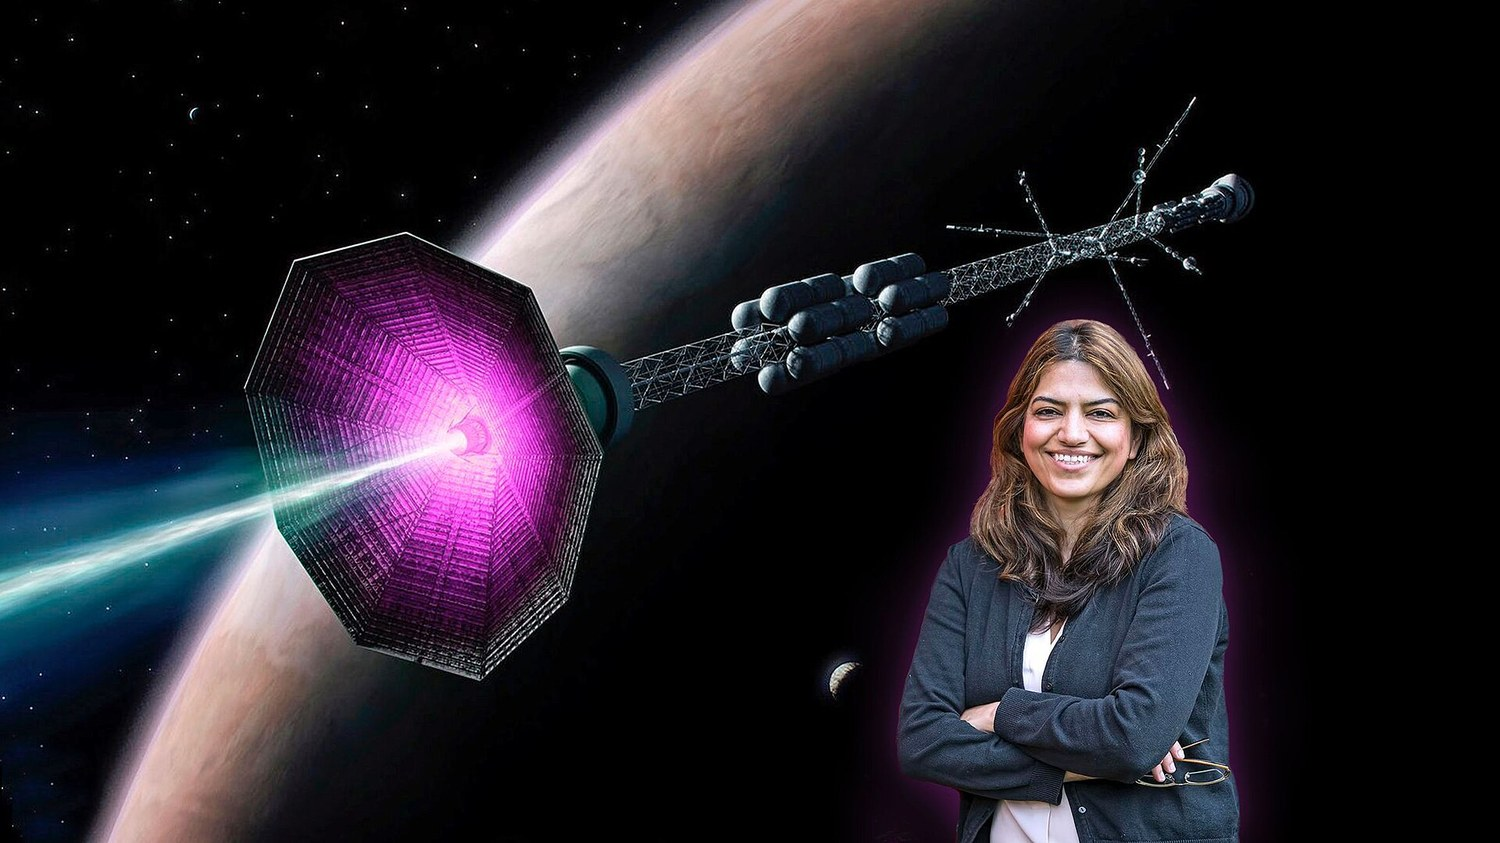
\includegraphics[width=0.72\textwidth]{../figures/o_pppl_fusion_rocket.jpg}
\caption{磁喷嘴不做静电加速：它让等离子体沿磁力线膨胀，把轴向动能直接变成推力。本节讲的比冲与功率账，就是这类「无栅极」推进方案的核心权衡。}
\label{fig:photo-appo3}
\figsource{Elle Starkman / PPPL，Public domain（Wikimedia Commons）}
\end{figure}

\section{磁喷嘴与 VASIMR：让比冲可调}

不用栅极也能加速：让等离子体在\textbf{发散磁场}（磁喷嘴）中膨胀，平行速度增加、垂直速度减小，最后由等离子体与磁场的“脱磁”把推力交出来。这类装置（如 VASIMR）通常用离子回旋共振加热（附录 M 的 ICRH）把功率交给离子，因此\textbf{比冲可以调}。

把 $P_{\mathrm{jet}}=\frac12Tv_{\mathrm{ex}}$ 与 $v_{\mathrm{ex}}=g_0I_{\mathrm{sp}}$ 联立，得到电推进的基本交换关系：
\begin{equation}
T=\frac{2\eta P_{\mathrm{in}}}{g_0I_{\mathrm{sp}}}
\qquad\Longrightarrow\qquad
T\propto\frac{P_{\mathrm{in}}}{I_{\mathrm{sp}}} .
\label{eq:app-o-triangle}
\end{equation}

\begin{table}[htbp]
\centering
\small
\caption{同一个 $200\ \mathrm{kW}$ 电源（$\eta=0.70$），比冲调高，推力就减半}
\label{tab:app-o-power}
\begin{tabular}{@{}rrrr@{}}
\toprule
$I_{\mathrm{sp}}$（$\mathrm{s}$） & $v_{\mathrm{ex}}$（$\mathrm{km/s}$） & $T$（$\mathrm{N}$） & $\dot m$（$\mathrm{mg/s}$） \\
\midrule
2000 & 19.6 & 14.3 & 727.9 \\
5000 & 49.0 & 5.71 & 116.5 \\
10000 & 98.1 & 2.86 & 29.1 \\
\bottomrule
\end{tabular}
\end{table}

与化学上面级对照：一台 $100\ \mathrm{kN}$ 量级的化学发动机推力是它的上万倍，但比冲只有 $1/10$。所以电推进的用法从来不是“起飞”，而是\textbf{入轨后的长期加速}：先把比冲调低换取推力（快速变轨），进入巡航后再把比冲调高（省推进剂）。

结论：\textbf{同一个电源，比冲调高一倍，推力就减半}——$T\propto1/I_{\mathrm{sp}}$ 是电推进无法回避的交换，也正是“可调比冲”的价值所在。

{\footnotesize
\textbf{出处：}Ahedo 的磁喷嘴与空间推进综述。
Chang D\'iaz 等的 VASIMR 论文（离子回旋加热与可调比冲）。
}


\section{中和、寿命与羽流：效率的损失清单}

\textbf{中和器。}离子束必须被等量电子中和，否则束自身电位会升到把电子拉回、把离子推回的量级。取 $I_e=I_b=2\ \mathrm{A}$、耦合电压约 $15\ \mathrm{V}$，中和器功耗 $I_e\Delta V=30\ \mathrm{W}$，只占 $2\ \mathrm{kW}$ 束功率的 $1.5\%$。

\textbf{电荷交换（CEX）侵蚀。}快离子与中性原子交换电荷后变成慢离子，慢离子被束电位加速、撞向栅极或通道壁（机制与附录 N \S N.4 的溅射侵蚀同源）。束路径 $L$ 上发生 CEX 的概率为
\begin{equation}
P_{\mathrm{CEX}}\approx n_n\sigma_{\mathrm{CEX}}L .
\label{eq:app-o-cex}
\end{equation}
取 $\sigma_{\mathrm{CEX}}=5\times10^{-19}\ \mathrm{m^2}$、$L=0.3\ \mathrm{m}$：$n_n=10^{17}\ \mathrm{m^{-3}}$ 时 $P_{\mathrm{CEX}}=1.5\%$，$n_n=10^{18}\ \mathrm{m^{-3}}$ 时升到 $15\%$——\textbf{中性密度差一个量级，寿命差一个量级}。

\textbf{羽流发散。}推力只取轴向分量，$T_{\mathrm{eff}}=T\cos\theta$：发散角 $15^\circ$ 损失 $3.4\%$，$25^\circ$ 损失 $9.4\%$。

\begin{table}[htbp]
\centering
\small
\caption{电推进的效率损失清单（$200\ \mathrm{kW}$ 级装置的典型量级）}
\label{tab:app-o-loss}
\begin{tabular}{@{}p{2.5cm}p{2.6cm}p{5.6cm}p{4.3cm}@{}}
\toprule
损失项 & 量级 & 物理原因 & 能否改进 \\
\midrule
放电损耗（电离/激发/阴极） & $35$--$50\%$ & 每产生一个氙离子至少付出 $12.13\ \mathrm{eV}$（占 $300\ \mathrm{V}$ 束能的 $4.0\%$、$1000\ \mathrm{V}$ 的 $1.2\%$），其余耗在激发、辐射与阴极 & \textbf{主项}：提高电压、优化放电室 \\
中和器 & $\approx1.5\%$ & 中和电子流 $I_e=I_b$，耦合电压约 $15\ \mathrm{V}$ & 空间很小 \\
CEX 侵蚀 & $1.5\%$（$n_n=10^{17}$）到 $15\%$（$n_n=10^{18}$） & 快离子与中性原子电荷交换，慢离子被加速撞向栅极/壁 & 降低中性密度、磁屏蔽（\textbf{决定寿命}） \\
羽流发散 & $3.4\%$（$15^\circ$）到 $9.4\%$（$25^\circ$） & 径向速度分量不贡献推力（$T_{\mathrm{eff}}=T\cos\theta$） & 离子光学设计（与栅极寿命相互牵制） \\
\bottomrule
\end{tabular}
\end{table}

结论：\textbf{电推进的效率天花板不在加速原理，而在损失清单}——放电损耗 $35$--$50\%$ 才是主项，其余所有工程努力都是围绕“把它压下去、同时不让寿命掉下来”。

{\footnotesize
\textbf{出处：}Goebel \& Katz 的推力器效率、空心阴极与羽流章节。
附录 N \S N.4 的溅射侵蚀口径。
}


\section{六道估算练习}


\begin{enumerate}
\item \textbf{（比冲与火箭方程）} 某电推进 $I_{\mathrm{sp}}=2500\ \mathrm{s}$。求排气速度；若任务需要 $\Delta v=6\ \mathrm{km/s}$，质量比 $m_0/m_f$ 是多少？\\
\textbf{答案：}$v_{\mathrm{ex}}=2500\times9.80665\approx2.45\times10^{4}\ \mathrm{m/s}=24.5\ \mathrm{km/s}$；$m_0/m_f=e^{6000/24517}\approx1.277$，即推进剂只占起飞质量的 $21.7\%$。

\item \textbf{（推力-功率账）} $T=0.2\ \mathrm{N}$、$I_{\mathrm{sp}}=2500\ \mathrm{s}$。求推进剂流量与射流功率；若整机效率 $0.55$，输入功率是多少？\\
\textbf{答案：}$\dot m=T/(g_0I_{\mathrm{sp}})=0.2/24517\approx8.16\times10^{-6}\ \mathrm{kg/s}=8.16\ \mathrm{mg/s}$；$P_{\mathrm{jet}}=\frac12Tv_{\mathrm{ex}}=0.5(0.2)(24517)\approx2452\ \mathrm{W}$；$P_{\mathrm{in}}=2452/0.55\approx4458\ \mathrm{W}$。

\item \textbf{（静电加速）} 氙离子束 $V_b=1200\ \mathrm{V}$、$I_b=4\ \mathrm{A}$。求离子速度、比冲、推力与射流功率。\\
\textbf{答案：}$v=\sqrt{2(1.602\times10^{-19})(1200)/2.180\times10^{-25}}\approx4.20\times10^{4}\ \mathrm{m/s}=42.0\ \mathrm{km/s}$，$I_{\mathrm{sp}}=4282\ \mathrm{s}$；$T=I_b\sqrt{2m_iV_b/q}=4\times0.05715\approx0.229\ \mathrm{N}$；$P_{\mathrm{jet}}=I_bV_b=4800\ \mathrm{W}$（验证：$\frac12Tv=0.5(0.229)(4.20\times10^{4})\approx4.8\times10^{3}\ \mathrm{W}$）。

\item \textbf{（空间电荷限制）} 用配套手册 K.7 的 Child--Langmuir 律，取 $V=1200\ \mathrm{V}$、$d=1\ \mathrm{mm}$、氙离子。求最大束流密度；若要引出 $3\ \mathrm{A}$，栅极面积至少多大？\\
\textbf{答案：}$j=\frac{4\varepsilon_0}{9}\sqrt{2q/m_i}\,V^{3/2}/d^2\approx198\ \mathrm{A/m^2}$；面积 $A=I_b/j=3/198\approx1.51\times10^{-2}\ \mathrm{m^2}=151\ \mathrm{cm^2}$。注意电压只涨 $20\%$（$1000\to1200\ \mathrm{V}$），电流密度涨 $31\%$。

\item \textbf{（霍尔推力器）} 通道内 $n_n=5\times10^{18}\ \mathrm{m^{-3}}$、$\sigma=3\times10^{-19}\ \mathrm{m^2}$、$T_e=25\ \mathrm{eV}$、$B=0.015\ \mathrm{T}$。求 $\omega_{ce}\tau_e$；再求放电电压 $250\ \mathrm{V}$ 时的比冲。\\
\textbf{答案：}$v_{th}=\sqrt{2k_BT_e/m_e}\approx2.97\times10^{6}\ \mathrm{m/s}$，$\nu_{en}=n_n\sigma v_{th}\approx4.45\times10^{6}\ \mathrm{s^{-1}}$，$\omega_{ce}=eB/m_e=2.64\times10^{9}\ \mathrm{rad/s}$，故 $\omega_{ce}\tau_e=\omega_{ce}/\nu_{en}\approx593\gg1$（电子被磁化）；\\
再由 $v_i=\sqrt{2qV/m_i}$（$V=250\ \mathrm{V}$）得 $v_i\approx1.92\times10^{4}\ \mathrm{m/s}$，$I_{\mathrm{sp}}=v_i/g_0\approx1955\ \mathrm{s}$。

\item \textbf{（磁喷嘴）} 一台 $300\ \mathrm{kW}$ 的磁喷嘴推力器，$I_{\mathrm{sp}}=4000\ \mathrm{s}$、$\eta=0.65$。求推力与推进剂流量；$1\ \mathrm{t}$ 推进剂能连续工作多少天？\\
\textbf{答案：}$T=2\eta P_{\mathrm{in}}/(g_0I_{\mathrm{sp}})=2(0.65)(3\times10^{5})/(9.80665\times4000)\approx9.94\ \mathrm{N}$；$\dot m=T/(g_0I_{\mathrm{sp}})\approx2.53\times10^{-4}\ \mathrm{kg/s}$；$1000\ \mathrm{kg}/2.53\times10^{-4}\ \mathrm{kg/s}\approx3.95\times10^{6}\ \mathrm{s}\approx45.7\ \mathrm{day}$。
\end{enumerate}


\section{来源、分级与版权说明}

\begingroup\small
本附录的数字都可以用 \texttt{tools/\allowbreak{}calc/\allowbreak{}appO\_calc.py} 重算一遍；脚本与当时的输出记录都在仓库里。

\begin{table}[htbp]
\centering
\small
\caption{本附录各节的取材与本书的处理方式}
\label{tab:app-o-source}
\begin{tabular}{@{}p{1.1cm}p{4.8cm}p{5.0cm}p{4.4cm}@{}}
\toprule
节 & 主要取材（经典教材与文献） & 借鉴的内容 & 本书的处理 \\
\midrule
O.1 & Sutton \& Biblarz《Rocket Propulsion Elements》第 9 版（火箭方程、比冲）；Jahn《Physics of Electric Propulsion》第 1 章 & 齐奥尔科夫斯基公式、比冲定义、推进方式分类 & 用四个自拟比冲值（$450$/$1800$/$3000$/$5000\ \mathrm{s}$）算同一 $\Delta v=10\ \mathrm{km/s}$ 的质量比表 \\
O.2 & Goebel \& Katz《Fundamentals of Electric Propulsion》的推力器指标章节 & $T=\dot mv_{\mathrm{ex}}$、$P_{\mathrm{jet}}=\frac12Tv_{\mathrm{ex}}$、效率与 $T/P$ 的关系 & 推出与推力无关的 $T/P_{\mathrm{in}}=2\eta/(g_0I_{\mathrm{sp}})$，并用公开级指标反算校核 \\
O.3 & 配套手册 K.7 的 Child--Langmuir 推导；Child (1911)、Langmuir (1913)；Goebel \& Katz 的离子光学章 & 单离子能量方程、束流推力 $T=I_b\sqrt{2m_iV_b/q}$、空间电荷限制 & 指出恒等式 $P_{\mathrm{jet}}=I_bV_b$，并用 $V^{3/2}$ 说明“面积比电压更重要” \\
O.4 & Choueiri 的电推进等离子体物理综述；Jahn 的 $\mathbf{E}\times\mathbf{B}$ 推力器章 & 磁化判据、霍尔电流、$\mathbf{E}\times\mathbf{B}$ 漂移、放电电压定比冲 & 用自拟参数（$B=0.02\ \mathrm{T}$、$n_n=10^{19}$、$V_d=300\ \mathrm{V}$）重算磁化程度与推力 \\
O.5 & Ahedo 的磁喷嘴与空间推进综述；Chang D\'iaz 等的 VASIMR 论文 & 磁喷嘴膨胀与脱磁、离子回旋加热、可调比冲 & 把“功率-推力-比冲”写成一条交换关系并制成同一电源的三档表 \\
O.6 & Goebel \& Katz 的效率、空心阴极与羽流章；附录 N \S N.4 的溅射口径 & 中和器、CEX 侵蚀、羽流发散损失 & 用一台 $200\ \mathrm{kW}$ 级的损失清单替代笼统的“效率”数字 \\
\bottomrule
\end{tabular}
\end{table}

\textbf{版权与独立性声明：}
\begin{itemize}
\item 本附录\textbf{不复制}任何教材或文献的题目原文、解答、图表与数据表；表格中的参数区间与物理结论属于教科书公共知识，文字表述与全部数值由本书自拟。
\item 表中列出的教材与文献是\textbf{取材来源}（说明该主题在哪本书里讲、按什么顺序讲），不是逐句引用；读者若要系统学习，请直接阅读原书。
\item 本附录所用的一切“文献量级输入”（$m_{\mathrm{Xe}}=131.29\ \mathrm{u}$、$B=0.02\ \mathrm{T}$、$n_n$ 与 $\sigma$ 的取值、$\eta=0.5$--$0.7$、$\sigma_{\mathrm{CEX}}=5\times10^{-19}\ \mathrm{m^2}$、发散角）都在正文中\textbf{显式标出}，便于读者替换成自己装置的数据重算；结论中依赖这些输入的倍数关系（如“霍尔电流是束流的 $28.6$ 倍”）会随输入变化，但量级结论稳定。
\item 本附录只给出可自行检索的书名、作者与年份，\textbf{不写无法核实的 DOI 与卷页}。
\end{itemize}

\begin{tip}{与配套手册 K、M、N 串联使用}{tip-appo-chain}
建议的用法：
\begin{enumerate}[nosep,leftmargin=1.6em]
  \item 先在配套手册 K 里把 Child--Langmuir 律（K.7）与鞘层加速（K.3）做一遍，那是本附录 \S O.3 的地基；
  \item 再读附录 M 的离子回旋加热，理解 \S O.5 的功率是怎么放进离子的；
  \item 最后做本附录的 6 道估算题，并把 \S O.6 的损失清单与附录 N 的溅射侵蚀对照着看——两边算的都是“离子撞壁”，只是一个要推力、一个怕寿命。
\end{enumerate}
\end{tip}
\endgroup
